\documentclass{article}

\usepackage{fullpage}
\usepackage{color}
\usepackage{amsmath}
\usepackage{url}
\usepackage{verbatim}
\usepackage{graphicx}
\usepackage{parskip}
\usepackage{amssymb}
\usepackage{nicefrac}
\usepackage{listings} % For displaying code
\usepackage{algorithm2e} % pseudo-code

\def\rubric#1{\gre{Rubric: \{#1\}}}{}

% Colors
\definecolor{blu}{rgb}{0,0,1}
\def\blu#1{{\color{blu}#1}}
\definecolor{gre}{rgb}{0,.5,0}
\def\gre#1{{\color{gre}#1}}
\definecolor{red}{rgb}{1,0,0}
\def\red#1{{\color{red}#1}}
\def\norm#1{\|#1\|}

% Math
\def\R{\mathbb{R}}
\def\argmax{\mathop{\rm arg\,max}}
\def\argmin{\mathop{\rm arg\,min}}
\newcommand{\mat}[1]{\begin{bmatrix}#1\end{bmatrix}}
\newcommand{\alignStar}[1]{\begin{align*}#1\end{align*}}
\def\half{\frac 1 2}

% LaTeX
\newcommand{\fig}[2]{\includegraphics[width=#1\textwidth]{#2}}
\newcommand{\centerfig}[2]{\begin{center}\includegraphics[width=#1\textwidth]{#2}\end{center}}
\def\items#1{\begin{itemize}#1\end{itemize}}
\def\enum#1{\begin{enumerate}#1\end{enumerate}}

\begin{document}


\title{CPSC 340 Assignment 5 (due Friday November 16 at 11:55pm)}
\date{}
\maketitle

\vspace{-7em}

\section{Kernel Logistic Regresion}

If you run \verb|python main.py -q 1| it will load a synthetic 2D data set, split it into train/validation sets, and then perform regular logistic regression and kernel logistic regression (both without an intercept term, for simplicity). You'll observe that the error values and plots generated look the same since the kernel being used is the linear kernel (i.e., the kernel corresponding to no change of basis).

\subsection{Implementing kernels}
Polynomial kernel:
Training error 0.183
Validation error 0.170\\
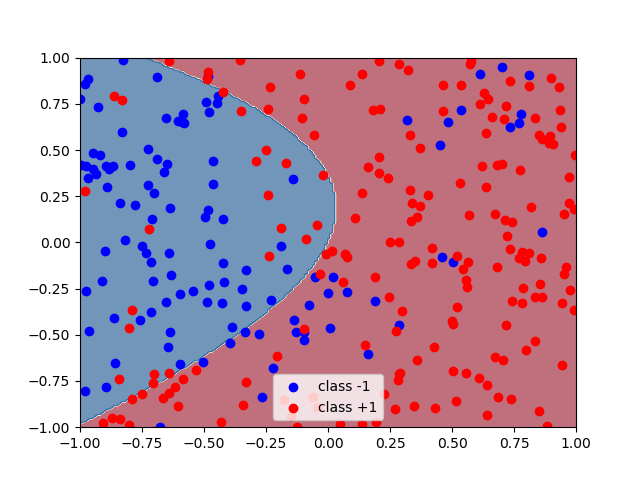
\includegraphics[scale=0.5]{logRegPolyKernel.png}\\

RBF Kernel: 
Training error 0.127
Validation error 0.090\\
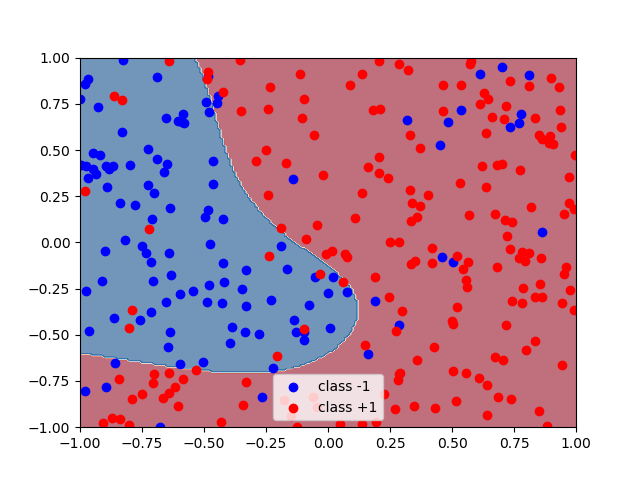
\includegraphics[scale=0.5]{logRegRBFKernel.png}\\

\subsection{Hyperparameter search}
For both training and validation error, I got $\lambda = 1$ and $\sigma = 100$.\\
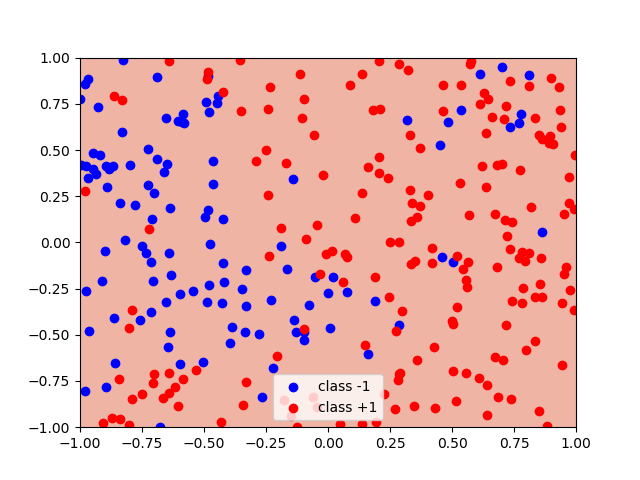
\includegraphics[scale=0.5]{RBFKernelT.png}\\
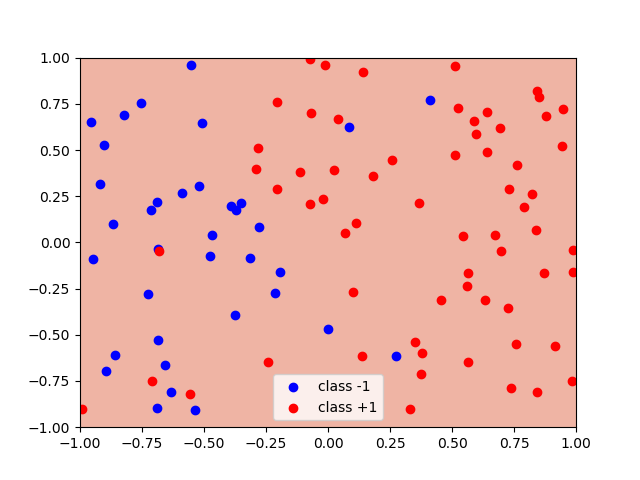
\includegraphics[scale=0.5]{RBFKernelVal.png}\\
\subsection{Reflection}
\rubric{reasoning:1}

Briefly discuss the best hyperparameters you found in the previous part, and their associated plots. Was the training error minimized by the values you expected, given the ways that $\sigma$ and $\lambda$ affect the fundamental tradeoff?


\section{MAP Estimation}
\begin{enumerate}
    \item $f(w) = ||Xw-y||_1 + \frac{1}{2\sigma^2}||w||^2 $
    \item $f(w) = \frac{1}{2}(Xw-y)^T\Sigma^{-1}(Xw-y)+\lambda||w||_1$
    \item The regularizer is $\frac{\lambda}{2}||w||^2$.
    \item 
\end{enumerate}

\section{Principal Component Analysis}
\begin{enumerate}
    \item We want to center the two variables around 0. $x_2$ is centered at 1. The centered $x_2$ is that all
    its points -1. Then, the centered variables lie along $-2x_1 = x_2$. Then the vector is (-2,1) and the magnitude
    is $\sqrt{(-2)^2+1^2} = \sqrt{5}$. Then the normalized vector is $(\frac{-2}{\sqrt{5}}, \frac{1}{\sqrt{5}})$.
    \item $$z = \frac{(-3-0)}{\sqrt{5}}+\frac{(2.5-1)}{\sqrt{5}} = \frac{-3}{2\sqrt{5}}$$
    $$\hat{x} = \frac{-3}{2\sqrt{5}}(\frac{-2}{\sqrt{5}}, \frac{1}{\sqrt{5}})+(0,1) = (\frac{3}{5},\frac{-3}{10})$$
    $$\text{error} = \sqrt{(\frac{3}{5}+3)^2+(\frac{-3}{10}-2.5)^2} = 4.5607$$
    \item $$z = \frac{(-3-0)}{\sqrt{5}}+\frac{(2-1)}{\sqrt{5}} = \frac{-2}{\sqrt{5}}$$
    $$\hat{x} = \frac{-2}{\sqrt{5}}(\frac{-2}{\sqrt{5}}, \frac{1}{\sqrt{5}})+(0,1) = (\frac{4}{5},\frac{-2}{5})$$
    $$\text{error} = \sqrt{(\frac{4}{5}+3)^2+(\frac{-2}{5}-2)^2} = 4.4944$$
\end{enumerate}

\section{PCA Generalizations}

\subsection{Robust PCA}
Code is in pca.py and figures are in figs folder.

\subsection{Reflection}
\rubric{reasoning:3}

\enum{
\item Briefly explain why using the L1 loss might be more suitable for this task than L2. 
\item How does the number of video frames and the size of each frame relate to $n$, $d$, and/or $k$?
\item What would the effect be of changing the threshold (see code) in terms of false positives (cars we identify that aren't really there) and false negatives (real cars that we fail to identify)?
}

\section{Very-Short Answer Questions}

\enum{
\item The "other" normal equations are faster when $d>n$ where the cost is $O(n^2k+n^3)$ instead of $O(nk^2+k^3)$.
\item An advantage for kernel k-means over normal k-means is that kernel k-means allows for non-convex clusters
\item MAP not only maximizes the likelihood but also the prior, $p(w)$ term which is the regularizer.
\item In generative model, we get $p(y_i|x_i)$ from using the rules of probability. For discriminitive model, $p(y_i|x_i)$
is modeled directly from fixed features. 
\item No. Higher k should generally have lower loss since it contains more dimensions so the loss is minimized. In some case,
higher k may result in the same loss (when all data points lie on w) but it should never be higher loss. 
\item Label Switching means that the ordering of vectos minimizing PCA may be different which can lead to non-unique solutions
\item $k$ is the number of dimensions/features we want. It wouldn't make sense for $k>d$ because then we would want more
features than we already have.
\item eigenfaces will be stored in $X$
\item Stochastic Descent has a cost of $O(k)$ per iteration which can be useful for large datasets but it does not enforce
uniqueness. 
\item $\alpha^t = 1/\sqrt{t}$.
\item Global features uses features to predict what is important to all examples while local features allow us to predict
what is important to a specific example.
}


\end{document}